% Template for the Journal of Computational Science and Applications (JCSA)
% Published by the University of Lahore -- ISSN 2710-3102
% Official author guidelines: https://journals.uol.edu.pk/JCSA/Author-Guideline
%
% v2 manuscript: Claude Haiku, GPT-4o-mini, Gemini Flash-Lite on 540 MMLU items × 5 trials.
% Numbers verified from data/v2/processed/*_v2.csv (stamp 20260716T175808Z).
\documentclass[twoside,twocolumn,10pt]{article}
\usepackage{fancyhdr}
\usepackage{geometry}
\usepackage{multicol}
\usepackage{abstract}
\usepackage{graphicx}
\usepackage{caption}
\usepackage{titlesec}
\usepackage{ragged2e}
\usepackage{amssymb}
\usepackage{parskip}
\usepackage{amsmath}
\usepackage{newtxtext}
\usepackage{booktabs}
\usepackage{array}
\usepackage{hyperref}
\usepackage{placeins}
\usepackage{verbatim}

\setcounter{page}{1}

\newcolumntype{L}[1]{>{\raggedright\arraybackslash}p{#1}}
\newcolumntype{C}[1]{>{\centering\arraybackslash}p{#1}}
\newcolumntype{R}[1]{>{\raggedleft\arraybackslash}p{#1}}

\usepackage[font=footnotesize, labelfont=bf, justification=raggedright, format=plain]{caption}

\captionsetup[table]{
    labelsep=period,
    justification=raggedright
}

\captionsetup[figure]{
    labelsep=period,
    justification=raggedright
}

\graphicspath{{figures/}{../figures/v2/}}

\geometry{
    a4paper,
    left=0.8in,
    right=0.8in,
    top=1in,
    bottom=1in
}

\setlength{\columnsep}{15pt}

\renewcommand{\abstractname}{\hspace{1.3em}\textbf{Abstract}}

\titleformat{\section}{\large\bfseries\uppercase}{\thesection.}{1em}{}
\titleformat{\subsection}{\normalfont\bfseries\flushleft}{\thesubsection.}{1em}{}
\titleformat{\subsubsection}{\normalfont\bfseries\itshape\flushleft}{\thesubsubsection}{1em}{}

\renewcommand{\abstractnamefont}{\normalfont\fontsize{14}{20}\bfseries}
\renewcommand{\absnamepos}{flushleft}
\renewcommand{\abstracttextfont}{\normalfont\fontsize{11}{13}\selectfont}

\newcommand{\keywordsname}{Keywords}
\newenvironment{keywords}
  {\par\noindent\hspace{2em}\textbf{\keywordsname:}}
  {\par}

\hyphenpenalty=10000
\exhyphenpenalty=10000
\sloppy

\pagestyle{fancy}
\fancyhf{}

\fancyhead[C]{\small Difficulty-Stratified Evaluation of Confidence Calibration in Large Language Models}
\fancyhead[CE]{\small Deshpande et al. (2026)}
\fancyfoot[C]{\thepage}

\fancypagestyle{firstpage}{
  \fancyhf{}
  \fancyhead[LO]{\small 2026}
  \fancyhead[RO]{\small}
  \fancyfoot[L]{\footnotesize Received: July 2026; Revised: ; Accepted:\\\textsuperscript{*}Corresponding Author: Yohan Deshpande \textless yohan.deshpande@example.com\textgreater}
   \fancyfoot[R]{\footnotesize \copyright\ 2026. Published by University of Lahore,\\\textsuperscript{*} under the CC-BY license }
  \renewcommand{\headrulewidth}{0.4pt}
  \renewcommand{\footrulewidth}{0.4pt}
}

\title{\fontsize{16}{20}\selectfont\textbf{Difficulty-Stratified Evaluation of Confidence Calibration in Large Language Models}}
\author{
    \fontsize{12}{14}\selectfont
    Yohan Deshpande\textsuperscript{1}, Akul Bajpai\textsuperscript{2}\\[1ex]
    \fontsize{12}{14}\selectfont
    \textsuperscript{1} Monroe Township High School, Monroe Township, United States \\
   \textsuperscript{2}Monroe Township High School, Monroe Township, United States
}
\date{}

\begin{document}

\twocolumn[
\begin{@twocolumnfalse}
\vspace{-0.5cm}
\raggedright

{\fontsize{11}{13}\selectfont{Research Article}}
\vspace{-0.8cm}

\maketitle

\thispagestyle{firstpage}
\begin{abstract}
\fontsize{11}{13}\selectfont
\vspace{1em}
\justifying
\textit{Large language models (LLMs) are increasingly deployed as decision-support systems, yet the fluency of their responses can mask substantial uncertainty. Although calibration is essential for trustworthy AI, limited student-accessible work has examined self-reported confidence across controlled task difficulty while comparing contemporary API models under a locked protocol. We evaluate Claude Haiku (Anthropic), GPT-4o-mini (OpenAI), and Gemini~3.1 Flash-Lite (Google) on an expanded, difficulty-stratified Massive Multitask Language Understanding (MMLU) bank of 540 multiple-choice questions (original 180 frozen items plus a 360-item content-disjoint supplement) spanning STEM, Social Sciences, and Humanities at easy, medium, and hard tiers fixed prior to evaluation. Each model completed five trials at temperature 0.3 (max 1024 output tokens) and provided both an answer and confidence estimate (0--100). With format-repair retries, parse success was 100\% (8{,}100/8{,}100). Calibration was evaluated using accuracy, overconfidence gap, Expected Calibration Error (ECE), bootstrap 95\% confidence intervals, and response-level difficulty regressions with Holm--Bonferroni correction. All models exhibited increasing overconfidence as difficulty increased, consistent directionally with the hard--easy effect in human judgment. Claude Haiku achieved the strongest calibration (89.5\% accuracy; ECE $= 0.033$) with slight overall underconfidence, while GPT-4o-mini (71.5\% accuracy; ECE $= 0.157$) and Gemini Flash-Lite (87.6\% accuracy; ECE $= 0.117$) were overconfident, especially on hard items. Gemini additionally showed confidence collapse (95.6\% of scores $\geq 95$). For GPT-4o-mini, verbal confidence correlated only weakly with answer-token probability ($r = 0.22$). Verbal confidence is therefore an imperfect reliability signal and should complement, not replace, verification and human oversight. Limitations include multiple-choice evaluation, verbal rather than fully internal confidence for Claude/Gemini, and omission of open-weight local models from this submission.}

\vspace{-0.1cm}
\noindent\textbf{Keywords}
 Large Language Models (LLMs), Confidence Calibration, Task Difficulty, MMLU, Expected Calibration Error (ECE), Hard--Easy Effect, GPT-4o-mini, Gemini, Claude Haiku.

\end{abstract}

\vspace{1cm}
\end{@twocolumnfalse}
]

\section{Introduction}

\fontsize{12}{14}\selectfont

Large language models (LLMs) are increasingly used as study aids, productivity assistants, and informal decision-support tools. Their responses are often fluent, coherent, and presented with an authoritative tone, which can encourage users to interpret them as reliable even when the underlying information is incorrect or uncertain. As these systems become more integrated into education, research, and professional workflows, understanding whether an LLM's expressed confidence accurately reflects its likelihood of being correct has become an important consideration for the development and deployment of trustworthy artificial intelligence.

Confidence calibration refers to the degree to which reported confidence aligns with observed accuracy. A well-calibrated system expresses high confidence when it is likely to be correct and lower confidence when uncertainty is warranted. In cognitive psychology, calibration has long been recognized as a fundamental aspect of human judgment, with confidence systematically varying according to task difficulty. People tend to overestimate their performance on difficult tasks while underestimating it on easier tasks, a phenomenon commonly referred to as the \textit{hard--easy effect} (Moore \& Healy, 2008). Kruger and Dunning (1999) further demonstrated that limited competence may be accompanied by limited insight into one's own performance, leading individuals to express confidence that exceeds their actual ability. These findings suggest that confidence should be interpreted in the context of task difficulty rather than as an absolute indicator of correctness.

Confidence calibration is also an essential property of machine learning systems. Guo et al. (2017) demonstrated that modern neural networks are frequently miscalibrated and introduced Expected Calibration Error (ECE), which has become a standard metric for quantifying the agreement between confidence and accuracy. Unlike many traditional machine learning models, LLMs can express confidence directly through natural language, allowing calibration to be evaluated using verbally reported confidence rather than internal probability estimates (Kadavath et al., 2022; Xiong et al., 2023). As LLMs become increasingly relied upon for information retrieval, learning, and decision support, it is important to determine whether these verbal confidence estimates remain reliable across varying levels of task difficulty.

The purpose of this study is to examine how task difficulty influences verbal confidence calibration in large language models. Specifically, this study evaluates Claude Haiku, GPT-4o-mini, and Gemini~3.1 Flash-Lite using an expanded, difficulty-stratified subset of the Massive Multitask Language Understanding (MMLU) benchmark (Hendrycks et al., 2021). The evaluation consists of multiple-choice questions spanning STEM, Social Sciences, and Humanities, organized into easy, medium, and hard difficulty tiers fixed prior to model evaluation. Each model is required to provide both an answer and an explicit confidence estimate using a constrained response format. Calibration is assessed using accuracy, the overconfidence gap, Expected Calibration Error, bootstrap confidence intervals, and response-level regressions of overconfidence on difficulty to determine whether verbal confidence becomes increasingly misaligned with correctness as task difficulty increases and whether these patterns resemble the difficulty-dependent confidence effects observed in human judgment.

By evaluating calibration as a function of task difficulty rather than overall performance alone, this study provides a controlled assessment of verbal confidence across three contemporary API language models under a common experimental framework. Understanding how confidence changes as questions become more challenging has practical implications for the use of LLMs in educational, professional, and decision-support settings, where users may rely on expressed confidence as an indicator of reliability.

\section{Literature Review}

\fontsize{12}{14}\selectfont

\textbf{Calibration in Large Language Models.}
Confidence calibration has long been recognized as an essential property of reliable machine learning systems because predictive confidence should correspond closely to empirical accuracy. Early work in natural language processing demonstrated that confidence estimates produced by neural language models are not always well aligned with correctness. Desai and Durrett (2020) found that pretrained Transformer models exhibited substantially poorer calibration when evaluated on out-of-domain data than on in-domain tasks. Jiang et al. (2021) examined generative question answering models and reported that these systems frequently produced overconfident predictions despite incorrect answers. Together, these studies established that strong predictive performance does not necessarily imply well-calibrated confidence, particularly under more challenging evaluation conditions.

\textbf{Verbal Confidence and Uncertainty Estimation.}
Unlike traditional neural networks, large language models can communicate uncertainty directly through natural language. Lin et al. (2022) demonstrated that language models can produce verbal confidence estimates that reasonably correspond to prediction accuracy without requiring access to internal probability distributions. Alternative approaches estimate uncertainty through multiple model generations rather than explicit self-report. Kuhn et al. (2023) introduced semantic entropy, and Farquhar et al. (2024) further demonstrated that semantic entropy provides an effective signal for detecting hallucinations. Although these methods provide informative measures of uncertainty, they generally require repeated sampling procedures that differ from the single confidence judgments presented to users during typical interactions.

\textbf{Metacognition and Self-Knowledge in Language Models.}
Yin et al. (2023) introduced the SelfAware benchmark to evaluate whether LLMs can recognize questions that are fundamentally unanswerable. Although prompting and instruction tuning improved performance, language models remained substantially less reliable than human participants in recognizing the limits of their knowledge. Recognizing when a question cannot be answered differs from accurately calibrating confidence across questions that remain answerable but vary systematically in difficulty.

\textbf{Human Trust in Language Model Confidence.}
Steyvers et al. (2025) demonstrated that people frequently overestimate the accuracy of language model responses and that longer or more detailed explanations can increase perceived reliability without improving actual correctness. Consequently, improving the calibration of communicated confidence has important implications for both model reliability and human--AI interaction.

\textbf{Research Gap.}
Collectively, this body of work demonstrates that language model confidence is frequently imperfect, particularly under more challenging evaluation conditions (Desai \& Durrett, 2020; Jiang et al., 2021). Verbally reported confidence provides a practical alternative to probability-based calibration for black-box models (Lin et al., 2022), while semantic uncertainty methods offer sampling-based approaches for uncertainty estimation (Kuhn et al., 2023; Farquhar et al., 2024). However, comparatively little attention has been given to how verbally reported confidence changes as task difficulty systematically increases across a standardized knowledge benchmark under a locked multi-model API protocol with response-level inference and provider-specific internal-probability availability.

\textbf{Purpose of the Present Study.}
The present study addresses this gap by evaluating verbal confidence calibration across predetermined levels of task difficulty using an expanded, difficulty-stratified MMLU bank. Claude Haiku, GPT-4o-mini, and Gemini~3.1 Flash-Lite are evaluated under a common answer-plus-confidence prompting protocol. Calibration is quantified using accuracy, the overconfidence gap, ECE, bootstrap intervals, and Holm-corrected response-level tests. Where available (GPT-4o-mini), verbal confidence is also compared with answer-token log-probabilities.

\section{Methodology}

\fontsize{12}{14}\selectfont

\textbf{Experimental Design.}
This study evaluated the calibration of verbally reported confidence in large language models using a controlled, difficulty-stratified evaluation protocol. Three API language models---Claude Haiku, GPT-4o-mini, and Gemini~3.1 Flash-Lite---were presented with the same frozen expanded subset of multiple-choice questions from MMLU and required to provide both an answer and an explicit confidence estimate. Calibration was evaluated both overall and across difficulty tiers fixed prior to evaluation.

\textbf{Question Bank.}
Evaluation questions were drawn from the test split of MMLU (Hendrycks et al., 2021) using the Hugging Face \texttt{cais/mmlu} dataset. Questions were restricted to three academic domains: STEM, Social Sciences, and Humanities (\texttt{config/domains.yaml}).

Each subject was assigned to one of three difficulty levels (easy, medium, or hard) using a difficulty mapping fixed prior to evaluation (\texttt{config/difficulty\_map.yaml}) based on published MMLU subject-level performance patterns rather than the performance of the evaluated models.

The evaluation bank comprises 540 items: (i)~an original 180-item set sampled with seed~42 (up to 20 questions per domain$\times$difficulty cell), frozen byte-for-byte under \texttt{data/v1\_frozen/}; and (ii)~a 360-item content-disjoint supplement sampled with seed~43 (\texttt{data/v2/bank\_supplement\_360.json}). The combined bank is \texttt{data/v2/bank\_full\_v2.json}. One true duplicate pair in the original bank (\texttt{q0060}/\texttt{q0073}) is retained for archival comparability and noted in Limitations.

\textbf{Evaluated Models.}
Three contemporary API models were evaluated under matched decoding conditions (Table~\ref{tab:models}). Open-weight local models (Llama~3.1, Mistral) were not collected in this submission.

\begin{table}[ht]
\centering
\caption{Language models evaluated in this study.}
\label{tab:models}
\resizebox{\columnwidth}{!}{
\begin{tabular}{lll}
\toprule
\textbf{Model} & \textbf{Access Method} & \textbf{Identifier} \\
\midrule
Claude Haiku & Anthropic API & \texttt{claude-haiku-4-5-20251001} \\
GPT-4o-mini & OpenAI API & \texttt{gpt-4o-mini} \\
Gemini Flash-Lite & Google Gemini API & \texttt{gemini-3.1-flash-lite} \\
\bottomrule
\end{tabular}
}
\end{table}

All generations used a temperature of 0.3 with a maximum output length of 1024 tokens. Each model completed five independent evaluation trials for every question, resulting in 8{,}100 planned responses (540 questions $\times$ 3 models $\times$ 5 trials). GPT-4o-mini requests additionally collected token log-probabilities for the answer letter. Source code is available at \href{https://github.com/yoyoyohan/llm-calibration-audit/tree/v2-phase2-clients}{GitHub (v2-phase2-clients)}.

\textbf{Confidence Elicitation.}
Every inference call used the same structured prompt. Each model was instructed to return only:

\begin{verbatim}
ANSWER: [A/B/C/D]
CONFIDENCE: [0-100]
\end{verbatim}

The prompt contained the question, four labeled choices, formatting instructions, and a valid response example. This constrained protocol minimized formatting variability and avoided chain-of-thought as a confound. The primary prompt is locked character-for-character from the earlier protocol; on parse failure, up to two repair retries append a short format-repair footer without rewriting the locked template.

\textbf{Response Parsing.}
Model outputs were automatically parsed for answer letter and integer confidence. With parse-repair retries, parse success was 100\% for all models (Table~\ref{tab:parse}). All 8{,}100 responses therefore entered the calibration analyses.

\begin{table}[ht]
\centering
\caption{Response parse rates by model.}
\label{tab:parse}
\resizebox{\columnwidth}{!}{
\begin{tabular}{lc}
\toprule
\textbf{Model} & \textbf{Parseable Responses} \\
\midrule
Claude Haiku & 2700 / 2700 (100.0\%) \\
GPT-4o-mini & 2700 / 2700 (100.0\%) \\
Gemini Flash-Lite & 2700 / 2700 (100.0\%) \\
\bottomrule
\end{tabular}
}
\end{table}

\textbf{Evaluation Metrics.}
Correctness was determined by comparison with the official MMLU answer key. Confidence values were normalized to $[0,1]$ by dividing by 100. Primary metrics were accuracy, mean confidence, overconfidence gap (mean confidence $-$ accuracy), and ECE with ten equally spaced bins.

To quantify difficulty dependence with adequate sample size, ordinary least squares regression was performed at the \emph{response level}: the dependent variable was the per-response overconfidence gap (normalized confidence minus correctness), and difficulty was coded numerically (easy $= 1$, medium $= 2$, hard $= 3$). Domain-specific ECE summaries were computed as secondary analyses. For GPT-4o-mini, Pearson correlation between verbal confidence and answer-token probability was computed, along with ECE under each confidence source.

\textbf{Statistical Analysis.}
Bootstrap 95\% confidence intervals (2{,}000 resamples) were computed for accuracy, overconfidence gap, and ECE. Six predeclared tests---slope $\neq 0$ and hard-minus-easy gap $> 0$, for each of three models---were corrected jointly using Holm--Bonferroni. Human hard--easy findings served only as a qualitative comparison.

\textbf{Reproducibility.}
Configurations, banks, processed results (\texttt{data/v2/processed/}), and figure scripts are included in the project repository. Analysis was produced by \texttt{src/analyze\_v2.py} on collection stamp \texttt{20260716T175808Z}.

\section{Results}

\fontsize{12}{14}\selectfont

All analyses include the full set of 8{,}100 successfully parsed responses. Overall metrics are presented in Table~\ref{tab:overall}; difficulty, domain, regression, and verbal-versus-internal analyses follow.

%%%%%%%%%%%%%%%%%%%%%%%%%%%%%%%%%%%%%%%%%%%%%%%%%%%%%%%
\textbf{Overall Performance}
%%%%%%%%%%%%%%%%%%%%%%%%%%%%%%%%%%%%%%%%%%%%%%%%%%%%%%%

\begin{table}[!htbp]
\centering
\caption{Overall performance metrics by model (bootstrap 95\% CIs).}
\label{tab:overall}
\resizebox{\columnwidth}{!}{
\begin{tabular}{lccccc}
\toprule
\textbf{Model} & \textbf{N} & \textbf{Accuracy} & \textbf{Mean Conf.} & \textbf{Gap} & \textbf{ECE} \\
\midrule
Claude Haiku & 2700 & 0.895 {[}0.883, 0.907{]} & 0.878 & $-0.017$ {[}$-0.027$, $-0.006${]} & 0.033 {[}0.023, 0.044{]} \\
GPT-4o-mini & 2700 & 0.715 {[}0.697, 0.731{]} & 0.871 & 0.156 {[}0.140, 0.173{]} & 0.157 {[}0.141, 0.175{]} \\
Gemini Flash-Lite & 2700 & 0.876 {[}0.863, 0.889{]} & 0.992 & 0.115 {[}0.104, 0.129{]} & 0.117 {[}0.104, 0.129{]} \\
\bottomrule
\end{tabular}
}
\end{table}

Table~\ref{tab:overall} summarizes accuracy, mean confidence, overconfidence gap, and ECE. Claude Haiku achieved the highest accuracy with the lowest calibration error and slight aggregate underconfidence. GPT-4o-mini showed the lowest accuracy and largest ECE. Gemini Flash-Lite was highly accurate but substantially overconfident because mean confidence remained near ceiling (0.992).

%%%%%%%%%%%%%%%%%%%%%%%%%%%%%%%%%%%%%%%%%%%%%%%%%%%%%%%
\textbf{Calibration Across Task Difficulty}
%%%%%%%%%%%%%%%%%%%%%%%%%%%%%%%%%%%%%%%%%%%%%%%%%%%%%%%

\begin{table}[!htbp]
\centering
\caption{Performance metrics by model and task difficulty.}
\label{tab:difficulty}
\resizebox{\columnwidth}{!}{
\begin{tabular}{llccccc}
\toprule
\textbf{Model} & \textbf{Difficulty} & \textbf{N} & \textbf{Accuracy} & \textbf{Mean Conf.} & \textbf{Gap} & \textbf{ECE} \\
\midrule
Claude Haiku & Easy   & 900 & 0.926 & 0.885 & $-0.041$ & 0.043 \\
Claude Haiku & Medium & 900 & 0.890 & 0.869 & $-0.021$ & 0.045 \\
Claude Haiku & Hard   & 900 & 0.869 & 0.880 & 0.011 & 0.037 \\
\midrule
GPT-4o-mini & Easy   & 900 & 0.847 & 0.874 & 0.028 & 0.036 \\
GPT-4o-mini & Medium & 900 & 0.783 & 0.870 & 0.086 & 0.088 \\
GPT-4o-mini & Hard   & 900 & 0.514 & 0.868 & 0.354 & 0.354 \\
\midrule
Gemini Flash-Lite & Easy   & 900 & 0.949 & 0.990 & 0.041 & 0.045 \\
Gemini Flash-Lite & Medium & 900 & 0.876 & 0.992 & 0.117 & 0.117 \\
Gemini Flash-Lite & Hard   & 900 & 0.804 & 0.993 & 0.189 & 0.189 \\
\bottomrule
\end{tabular}
}
\end{table}

\begin{figure}[!htbp]
\centering

\includegraphics[width=\columnwidth]{figure2_overconfidence_by_difficulty.png}
\caption{Overconfidence gap across task difficulty levels (v2; predetermined subject tiers).}
\label{fig:difficulty_overconfidence}
\end{figure}

Table~\ref{tab:difficulty} and Figure~\ref{fig:difficulty_overconfidence} show calibration across difficulty. For all three models, the overconfidence gap rises from easy to hard. The increase is steepest for GPT-4o-mini (gap $0.028 \rightarrow 0.354$), driven by a large accuracy drop on hard items while mean confidence remains nearly flat. Gemini's gap also rises ($0.041 \rightarrow 0.189$) despite near-ceiling confidence at every tier. Claude remains closest to zero throughout, moving from mild underconfidence on easy items to slight overconfidence on hard items.

%%%%%%%%%%%%%%%%%%%%%%%%%%%%%%%%%%%%%%%%%%%%%%%%%%%%%%%
\textbf{Confidence Dispersion}
%%%%%%%%%%%%%%%%%%%%%%%%%%%%%%%%%%%%%%%%%%%%%%%%%%%%%%%

\begin{table}[!htbp]
\centering
\caption{Confidence dispersion by model (0--100 scale).}
\label{tab:dispersion}
\resizebox{\columnwidth}{!}{
\begin{tabular}{lccc}
\toprule
\textbf{Model} & \textbf{Mean} & \textbf{SD} & \textbf{\% $\geq$ 95} \\
\midrule
Claude Haiku & 87.8 & 13.4 & 42.6\% \\
GPT-4o-mini & 87.1 & 3.6 & 4.9\% \\
Gemini Flash-Lite & 99.2 & 2.5 & 95.6\% \\
\bottomrule
\end{tabular}
}
\end{table}

Gemini Flash-Lite exhibits \emph{confidence collapse}: near-ceiling mean confidence with very low dispersion (Table~\ref{tab:dispersion}). Rising overconfidence for Gemini is therefore driven primarily by falling accuracy rather than informative modulation of stated confidence.

%%%%%%%%%%%%%%%%%%%%%%%%%%%%%%%%%%%%%%%%%%%%%%%%%%%%%%%
\textbf{Domain-Level Performance}
%%%%%%%%%%%%%%%%%%%%%%%%%%%%%%%%%%%%%%%%%%%%%%%%%%%%%%%

\begin{table}[!htbp]
\centering
\caption{Expected calibration error by model and domain.}
\label{tab:domain}
\resizebox{\columnwidth}{!}{
\begin{tabular}{llcc}
\toprule
\textbf{Model} & \textbf{Domain} & \textbf{ECE} & \textbf{N} \\
\midrule
Claude Haiku & Humanities       & 0.047 & 900 \\
Claude Haiku & STEM             & 0.012 & 900 \\
Claude Haiku & Social Science   & 0.057 & 900 \\
\midrule
GPT-4o-mini & Humanities       & 0.156 & 900 \\
GPT-4o-mini & STEM             & 0.247 & 900 \\
GPT-4o-mini & Social Science   & 0.087 & 900 \\
\midrule
Gemini Flash-Lite & Humanities       & 0.128 & 900 \\
Gemini Flash-Lite & STEM             & 0.141 & 900 \\
Gemini Flash-Lite & Social Science   & 0.081 & 900 \\
\bottomrule
\end{tabular}
}
\end{table}

\begin{figure}[!htbp]
\centering

\includegraphics[width=\columnwidth]{figure3_ece_domain_heatmap.png}
\caption{ECE heatmap by model and domain (v2; lower is better).}
\label{fig:ece_heatmap_domain}
\end{figure}

Claude Haiku maintains low ECE across domains (Table~\ref{tab:domain}; Figure~\ref{fig:ece_heatmap_domain}). GPT-4o-mini shows the largest domain ECE on STEM (0.247). Gemini is intermediate across domains.

\FloatBarrier

%%%%%%%%%%%%%%%%%%%%%%%%%%%%%%%%%%%%%%%%%%%%%%%%%%%%%%%
\textbf{Reliability Diagrams and Capability Scatter}
%%%%%%%%%%%%%%%%%%%%%%%%%%%%%%%%%%%%%%%%%%%%%%%%%%%%%%%

\begin{figure}[!htbp]
\centering

\includegraphics[width=\columnwidth]{figure1_reliability_diagrams.png}
\caption{Reliability diagrams comparing verbal confidence calibration (v2).}
\label{fig:reliability}
\end{figure}

\begin{figure}[!htbp]
\centering
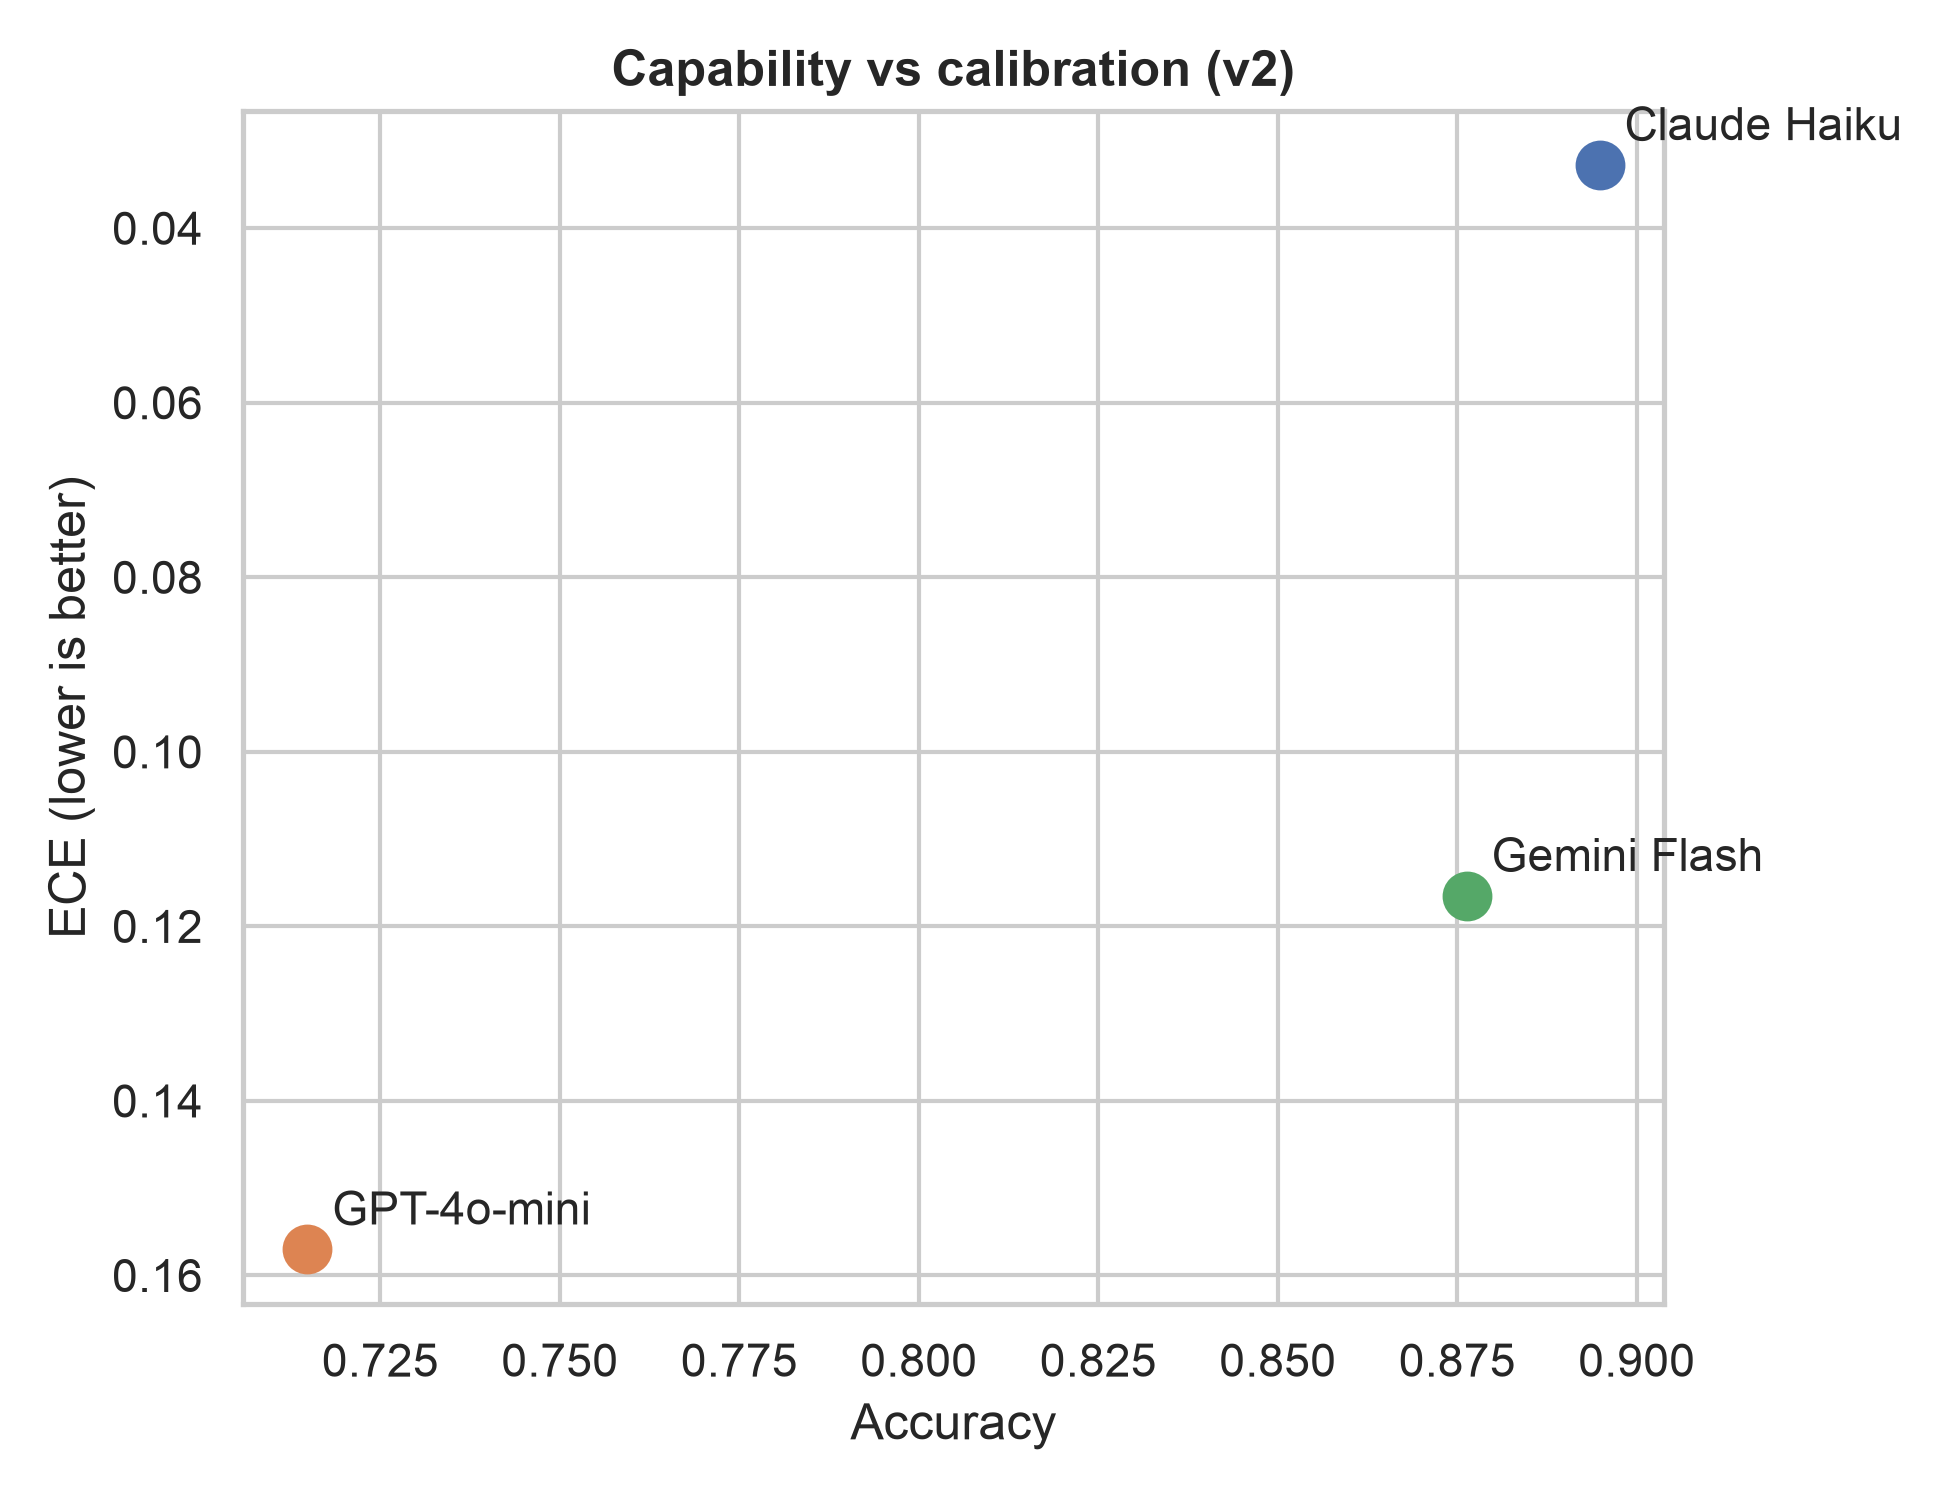
\includegraphics[width=\columnwidth]{figure4_accuracy_vs_ece.png}
\caption{Accuracy versus ECE across evaluated models (v2).}
\label{fig:acc_ece}
\end{figure}

Figure~\ref{fig:reliability} shows reliability diagrams. Claude Haiku remains closest to the ideal diagonal. GPT-4o-mini and Gemini deviate more, consistent with higher ECE. Figure~\ref{fig:acc_ece} summarizes the capability--calibration relationship in this three-model sample: higher accuracy tracks lower ECE, with Claude best on both axes and GPT-4o-mini worst.

\FloatBarrier

%%%%%%%%%%%%%%%%%%%%%%%%%%%%%%%%%%%%%%%%%%%%%%%%%%%%%%%
\textbf{Response-Level Difficulty Regression}
%%%%%%%%%%%%%%%%%%%%%%%%%%%%%%%%%%%%%%%%%%%%%%%%%%%%%%%

\begin{table}[!htbp]
\centering
\caption{Response-level OLS of per-response overconfidence gap on difficulty (easy$=$1, medium$=$2, hard$=$3), with Holm-corrected $p$-values.}
\label{tab:slopes}
\resizebox{\columnwidth}{!}{
\begin{tabular}{lcccccc}
\toprule
\textbf{Model} & \textbf{N} & \textbf{Slope} & \textbf{SE} & \textbf{95\% CI} & \textbf{$p$ (Holm)} & \textbf{$R^2$} \\
\midrule
Claude Haiku & 2700 & 0.026 & 0.007 & {[}0.013, 0.039{]} & $7.8\times10^{-5}$ & 0.006 \\
GPT-4o-mini & 2700 & 0.163 & 0.010 & {[}0.143, 0.183{]} & $3.1\times10^{-56}$ & 0.089 \\
Gemini Flash-Lite & 2700 & 0.074 & 0.008 & {[}0.059, 0.088{]} & $7.3\times10^{-22}$ & 0.034 \\
\bottomrule
\end{tabular}
}
\end{table}

Unlike three-point cell-mean regressions, Table~\ref{tab:slopes} uses all responses. Difficulty significantly predicted overconfidence for all three models after Holm correction. Effect sizes are modest for Claude ($R^2 = 0.006$) and larger for GPT-4o-mini ($R^2 = 0.089$). Hard-minus-easy gap contrasts were likewise significant after Holm correction for every model.

%%%%%%%%%%%%%%%%%%%%%%%%%%%%%%%%%%%%%%%%%%%%%%%%%%%%%%%
\textbf{Verbal versus Internal Confidence (GPT-4o-mini)}
%%%%%%%%%%%%%%%%%%%%%%%%%%%%%%%%%%%%%%%%%%%%%%%%%%%%%%%

\begin{table}[!htbp]
\centering
\caption{Verbal versus answer-token internal probability (GPT-4o-mini only).}
\label{tab:verbal_internal}
\resizebox{\columnwidth}{!}{
\begin{tabular}{lc}
\toprule
\textbf{Metric} & \textbf{Value} \\
\midrule
$N$ with internal prob. & 2700 \\
Pearson $r$ (verbal, internal) & 0.222 \\
ECE (verbal) & 0.157 \\
ECE (internal answer prob.) & 0.243 \\
\bottomrule
\end{tabular}
}
\end{table}

For GPT-4o-mini, verbal confidence and answer-token probability are positively but weakly correlated (Table~\ref{tab:verbal_internal}). ECE using internal answer probability is \emph{worse} than ECE using verbal confidence on this protocol. Claude and Gemini are excluded because Anthropic's public API does not expose token log-probabilities, and Gemini returned only aggregate \texttt{avgLogprobs} rather than per-token answer probabilities.

%%%%%%%%%%%%%%%%%%%%%%%%%%%%%%%%%%%%%%%%%%%%%%%%%%%%%%%
\textbf{Robustness: Original 180 versus Full 540}
%%%%%%%%%%%%%%%%%%%%%%%%%%%%%%%%%%%%%%%%%%%%%%%%%%%%%%%

\begin{table}[!htbp]
\centering
\caption{Original-180 subset versus full-540 bank (accuracy / gap / ECE).}
\label{tab:robust}
\resizebox{\columnwidth}{!}{
\begin{tabular}{llccc}
\toprule
\textbf{Bank} & \textbf{Model} & \textbf{Acc.} & \textbf{Gap} & \textbf{ECE} \\
\midrule
original\_180 & Claude Haiku & 0.911 & $-0.020$ & 0.037 \\
full\_540 & Claude Haiku & 0.895 & $-0.017$ & 0.033 \\
original\_180 & GPT-4o-mini & 0.726 & 0.148 & 0.152 \\
full\_540 & GPT-4o-mini & 0.715 & 0.156 & 0.157 \\
original\_180 & Gemini Flash-Lite & 0.874 & 0.117 & 0.119 \\
full\_540 & Gemini Flash-Lite & 0.876 & 0.115 & 0.117 \\
\bottomrule
\end{tabular}
}
\end{table}

Direction and ranking of calibration are stable under bank expansion (Table~\ref{tab:robust}).

\section{Discussion}

The primary empirical finding is that all three evaluated models exhibit increased overconfidence as task difficulty increases (Table~\ref{tab:difficulty}; Figure~\ref{fig:difficulty_overconfidence}). Although accuracy declines on harder questions, reported confidence does not decrease proportionally, producing larger confidence--accuracy discrepancies precisely where performance is weakest. Claude Haiku follows the same directional trend but with much smaller magnitude, remaining near-calibrated overall (ECE $= 0.033$; gap $= -0.017$).

Substantial differences emerge across models. Claude combines high accuracy (0.895) with the best calibration. GPT-4o-mini has lower accuracy (0.715) and the steepest response-level difficulty slope (0.163), with hard-tier gap reaching 0.354. Gemini is highly accurate (0.876) yet overconfident (gap $= 0.115$; ECE $= 0.117$) because confidence remains near ceiling with very low dispersion---a pattern better described as confidence collapse than as informative metacognitive modulation (Table~\ref{tab:dispersion}).

Because all three arms are API models, we do \emph{not} attribute calibration differences to open-weight versus proprietary architecture. In this sample, calibration tracks capability (Figure~\ref{fig:acc_ece}), with provider and model class confounded with accuracy.

The observed difficulty--overconfidence relationship is directionally consistent with human hard--easy research (Moore \& Healy, 2008) but should not be interpreted as evidence that LLMs share human metacognitive mechanisms (Kruger \& Dunning, 1999). The empirical parallel is narrower: as evaluation difficulty increases, model confidence becomes less aligned with correctness.

The GPT-4o-mini verbal-versus-internal comparison further cautions against treating either signal as a complete reliability measure: the two are only weakly correlated, and internal answer-token probabilities were not better calibrated than verbal reports under this elicitation protocol (Table~\ref{tab:verbal_internal}).

Practically, a reported confidence score is attractive but model-dependent. For Claude Haiku, verbal confidence is comparatively informative. For GPT-4o-mini on hard items and for Gemini's near-ceiling scores, high confidence frequently co-occurs with error. Confidence estimates should therefore complement external verification, especially on difficult STEM tasks.

\section{Limitations}

Evaluation is restricted to multiple-choice MMLU items; findings may not generalize to open-ended generation or tool-augmented agents. Difficulty is assigned via a subject-level mapping fixed prior to evaluation rather than item-level IRT. The original 180-item bank contains one true duplicate pair (\texttt{q0060}/\texttt{q0073}).

Confidence is primarily verbal (0--100). Internal answer-token probabilities were available only for GPT-4o-mini; Claude and Gemini are excluded from that comparison by API design, not by silent data loss. Constrained \texttt{ANSWER}/\texttt{CONFIDENCE} formatting suppresses chain-of-thought and may affect absolute accuracy relative to CoT-style leaderboards; claims concern miscalibration under this protocol.

Open-weight local models were not collected in this submission. No formal human-subjects baseline is included. Results are specific to temperature 0.3, five trials, max 1024 output tokens, the 540-item bank, and July 2026 model versions.

\section{Future Work}

Future work should extend to MMLU-Pro, GPQA, and related harder benchmarks; reintroduce open-weight local models under the same locked protocol; expand item-level difficulty estimation; systematically compare elicitation strategies; and connect calibration metrics to human reliance behavior. Where providers expose token probabilities, verbal-versus-internal comparisons should be repeated across model families.

\section{Conclusion}

Under a locked verbal confidence protocol on an expanded 540-item MMLU bank with five trials per item, Claude Haiku, GPT-4o-mini, and Gemini~3.1 Flash-Lite all show rising overconfidence with predetermined difficulty. Claude remains near-calibrated; GPT-4o-mini shows the steepest difficulty-linked overconfidence; Gemini combines high accuracy with confidence collapse. Verbal confidence is therefore not a universally reliable indicator of correctness and should be treated as a supporting signal rather than a substitute for verification. Calibration must be evaluated where models are most likely to fail---on hard items---not only where average performance appears strong.

\subsection*{Figures and Tables}

\begin{itemize}
    \item \textbf{Figure~\ref{fig:reliability}:} Reliability diagrams.
    \item \textbf{Figure~\ref{fig:difficulty_overconfidence}:} Overconfidence by difficulty.
    \item \textbf{Figure~\ref{fig:ece_heatmap_domain}:} Domain ECE heatmap.
    \item \textbf{Figure~\ref{fig:acc_ece}:} Accuracy versus ECE.
    \item \textbf{Table~\ref{tab:models}:} Evaluated models.
    \item \textbf{Table~\ref{tab:parse}:} Parse rates (100\%).
    \item \textbf{Table~\ref{tab:overall}:} Overall metrics with bootstrap CIs.
    \item \textbf{Table~\ref{tab:difficulty}:} Metrics by difficulty.
    \item \textbf{Table~\ref{tab:dispersion}:} Confidence dispersion / collapse.
    \item \textbf{Table~\ref{tab:domain}:} Domain ECE.
    \item \textbf{Table~\ref{tab:slopes}:} Response-level difficulty regression.
    \item \textbf{Table~\ref{tab:verbal_internal}:} Verbal vs internal (GPT-4o-mini).
    \item \textbf{Table~\ref{tab:robust}:} Original-180 vs full-540 robustness.
\end{itemize}

\renewcommand{\refname}{REFERENCES}

\begin{thebibliography}{99}

\bibitem{desai2020}
Desai, S., \& Durrett, G. (2020).
\textit{Calibration of Pre-trained Transformers}.
arXiv preprint arXiv:2003.07892.
https://arxiv.org/abs/2003.07892

\bibitem{farquhar2024semantic}
Farquhar, S., Kossen, J., Kuhn, L., \& Gal, Y. (2024).
Detecting hallucinations in large language models using semantic entropy.
\textit{Nature, 630}(8017), 625--630.
https://doi.org/10.1038/s41586-024-07421-0

\bibitem{guo2017calibration}
Guo, C., Pleiss, G., Sun, Y., \& Weinberger, K. Q. (2017).
\textit{On Calibration of Modern Neural Networks}.
arXiv preprint arXiv:1706.04599.
https://arxiv.org/pdf/1706.04599

\bibitem{hendrycks2021mmlu}
Hendrycks, D., Burns, C., Basart, S., Zou, A., Mazeika, M., Song, D., \& Steinhardt, J. (2021).
\textit{Measuring Massive Multitask Language Understanding}.
arXiv preprint arXiv:2009.03300.
https://arxiv.org/pdf/2009.03300

\bibitem{jiang2021calibration}
Jiang, Z., Araki, J., Ding, H., \& Neubig, G. (2021).
\textit{How Can We Know When Language Models Know? On the Calibration of Language Models for Question Answering}.
arXiv preprint arXiv:2012.00955.
https://doi.org/10.48550/arXiv.2012.00955

\bibitem{kadavath2022know}
Kadavath, S., Conerly, T., Askell, A., Henighan, T., Drain, D., Perez, E., Schiefer, N., Hatfield-Dodds, Z., Dassarma, N., Tran-Johnson, E., Johnston, S., El-Showk, S., Jones, A., Elhage, N., Hume, T., Chen, A., Bai, Y., Bowman, S., Fort, S., \& Kaplan, J. (2022).
\textit{Language Models (Mostly) Know What They Know}.
arXiv preprint arXiv:2207.05221.
https://arxiv.org/pdf/2207.05221

\bibitem{kruger1999unskilled}
Kruger, J., \& Dunning, D. (1999).
Unskilled and Unaware of It: How Difficulties in Recognizing One's Own Incompetence Lead to Inflated Self-Assessments.
\textit{Journal of Personality and Social Psychology, 77}(6), 1121--1134.
https://doi.org/10.1037/0022-3514.77.6.1121

\bibitem{kuhn2023semantic}
Kuhn, L., Gal, Y., \& Farquhar, S. (2023).
\textit{Semantic Uncertainty: Linguistic Invariances for Uncertainty Estimation in Natural Language Generation}.
arXiv preprint arXiv:2302.09664.
https://arxiv.org/abs/2302.09664

\bibitem{lin2022uncertainty}
Lin, S., Hilton, J., \& Evans, O. (2022).
\textit{Teaching Models to Express Their Uncertainty in Words}.
arXiv preprint arXiv:2205.14334.
https://arxiv.org/abs/2205.14334

\bibitem{moore2008overconfidence}
Moore, D. A., \& Healy, P. J. (2008).
The Trouble with Overconfidence.
\textit{Psychological Review, 115}(2), 502--517.
https://doi.org/10.1037/0033-295X.115.2.502

\bibitem{steyvers2025knowledge}
Steyvers, M., Tejeda, H., Kumar, A., Belem, C., Karny, S., Hu, X., Mayer, L. W., \& Smyth, P. (2025).
What large language models know and what people think they know.
\textit{Nature Machine Intelligence, 7}.
https://doi.org/10.1038/s42256-024-00976-7

\bibitem{xiong2023uncertainty}
Xiong, M., Hu, Z., Lu, X., Li, Y., Fu, J., He, J., \& Hooi, B. (2023).
\textit{Can LLMs Express Their Uncertainty? An Empirical Evaluation of Confidence Elicitation in LLMs}.
arXiv preprint arXiv:2306.13063 (ICLR 2024).
https://arxiv.org/abs/2306.13063

\bibitem{yin2023dontknow}
Yin, Z., Sun, Q., Guo, Q., Wu, J., Qiu, X., \& Huang, X. (2023).
\textit{Do Large Language Models Know What They Don't Know?}
In \textit{Findings of the Association for Computational Linguistics: ACL 2023}, 8653--8665.
https://aclanthology.org/2023.findings-acl.551.pdf

\end{thebibliography}

\end{document}
